% Created 2022-01-25 Tue 14:40
% Intended LaTeX compiler: pdflatex
\documentclass[11pt]{article}
\usepackage[utf8]{inputenc}
\usepackage[T1]{fontenc}
\usepackage{graphicx}
\usepackage{longtable}
\usepackage{wrapfig}
\usepackage{rotating}
\usepackage[normalem]{ulem}
\usepackage{amsmath}
\usepackage{amssymb}
\usepackage{capt-of}
\usepackage{hyperref}
\usepackage{color}
\usepackage{listings}
\usepackage{color}
\usepackage{listings}
\author{Maikol Solís}
\date{2022-01-25}
\title{Emacs workshop 2022: Day 2}
\hypersetup{
 pdfauthor={Maikol Solís},
 pdftitle={Emacs workshop 2022: Day 2},
 pdfkeywords={},
 pdfsubject={},
 pdfcreator={Emacs 27.2 (Org mode 9.6)}, 
 pdflang={English}}
\makeatletter
\newcommand{\citeprocitem}[2]{\hyper@linkstart{cite}{citeproc_bib_item_#1}#2\hyper@linkend}
\makeatother

\usepackage[notquote]{hanging}
\begin{document}


\section{Primero}
\label{sec:orgfa9dcad}
\subsection{Segundo}
\label{sec:org39abc7e}
\begin{enumerate}
\item Tercero
\label{sec:orga3599a8}
\end{enumerate}

\section{More examples of org-mode}
\label{sec:orgaf866f5}

\subsection{Captures and Templates}
\label{sec:org5730ff2}
\begin{verbatim}
(setq org-capture-templates
            '(("t" "Mi nueva tarea" entry
               ;; (file "~/documents/2022/2022_01_Taller_Emacs/Day_3/gtd.org")
               (file+headline "~/documents/2022/2022_01_Taller_Emacs/Day_3/gtd.org" "Bandeja de entrada")
               "* TODO %?\n  %i")
              ("j" "Journal" entry
               (file+datetree  "~/documents/2022/2022_01_Taller_Emacs/Day_3/journal.org")
               "* %?\nEntered on %U\n  %i\n  %a")))
\end{verbatim}



\url{https://orgmode.org/manual/Capture-templates.html}

\subsection{Agenda views}
\label{sec:org1bf3789}


\begin{verbatim}
(setq org-agenda-files '("~/documents/2022/2022_01_Taller_Emacs/Day_3/gtd.org"))
\end{verbatim}


\begin{verbatim}
  (setq org-agenda-custom-commands
        '(("z" "Mi propia agenda"
           (
            ;; (agenda "")
            (agenda "" ((org-agenda-start-day nil) ;nil
                        (org-agenda-span 0))) ;0
            (todo "WAIT" nil)
            (tags-todo "+PRIORITY=\"A\"+TODO=\"NEXT\"")))))
\end{verbatim}


\url{https://orgmode.org/manual/Custom-Agenda-Views.html}

\section{Export files}
\label{sec:org18b6371}

\subsection{Citations}
\label{sec:orgba002f6}

\begin{enumerate}
\item Zotero
\label{sec:orgad15fc3}
\begin{enumerate}
\item Zotero styles
\label{sec:orgbcc8850}
\begin{verbatim}
(setq org-cite-csl-styles-dir "~/Zotero/styles")
\end{verbatim}
\end{enumerate}

\item Setting Bibliography
\label{sec:org3745a45}
\begin{enumerate}
\item In \texttt{config.el} file
\label{sec:org41b3424}
\begin{verbatim}
(setq org-cite-global-bibliography
      '("~/Dropbox/home/documents/2022/2022_01_Taller_Emacs/Day_3/library.bib"))
\end{verbatim}
\item In-buffer
\label{sec:org4720b44}
\begin{verbatim}
#+BIBLIOGRAPHY: library.bib
\end{verbatim}
\end{enumerate}

\item Bibliographic Styles
\label{sec:org513a143}

By default is Chicago style.

\begin{description}
\item[{In parenthesis}] This work was already done \citeprocitem{1}{[1]}–\citeprocitem{4}{[4]}
\item[{In text:}] In \citeprocitem{4}{[4]}, \citeprocitem{5}{[5, p. 7]}, \citeprocitem{6}{[6]} we have \ldots{}
\item[{Only authors:}] The work of \citeprocitem{5}{[5]}\ldots{} In fact, \citeprocitem{5}{[5]} discovered that\ldots{}
\item[{Full list of styles:}] \url{https://blog.tecosaur.com/tmio/2021-07-31-citations.html}
\end{description}


\begin{enumerate}
\item References
\label{sec:org16ddd46}

\hypertarget{citeproc_bib_item_1}{[1] G. Sanchez, \textit{PLS Path Modeling with R}. Trowchez Editions, 2013.}

\hypertarget{citeproc_bib_item_2}{[2] C. R. Rao, Ed., \textit{Data mining and data visualization}, 1. ed. Amsterdam Heidelberg: Elsevier, North-Holland, 2005.}

\hypertarget{citeproc_bib_item_3}{[3] W. Härdle and L. Simar, \textit{Applied multivariate statistical analysis}, Fifth edition. Cham, Switzerland: Springer, 2019.}

\hypertarget{citeproc_bib_item_4}{[4] H. E. A. Tinsley and S. D. Brown, Eds., \textit{Handbook of applied multivariate statistics and mathematical modeling}. San Diego: Academic Press, 2000.}

\hypertarget{citeproc_bib_item_5}{[5] W. K. Härdle and Z. e. Hlávka, \textit{Multivariate Statistics: Exercises and Solutions}, 2nd ed. 2015. Berlin, Heidelberg: Springer Berlin Heidelberg : Imprint: Springer, 2015. doi: \href{https://doi.org/10.1007/978-3-642-36005-3}{10.1007/978-3-642-36005-3}.}

\hypertarget{citeproc_bib_item_6}{[6] J. F. Hair, \textit{Multivariate data analysis}, Eighth edition. Andover, Hampshire: Cengage, 2019.}
\end{enumerate}
\end{enumerate}


\section{org-babel}
\label{sec:org77d8fcc}

\subsection{Default block}
\label{sec:org48609dd}

\begin{verbatim}
print("hello world")
\end{verbatim}

\subsection{Exporting results}
\label{sec:org8976c7f}

\begin{verbatim}
print("hello world")
\end{verbatim}

\begin{verbatim}
hello world
\end{verbatim}

\subsection{Different kind of languages}
\label{sec:orgc9a9935}


\begin{enumerate}
\item Python
\label{sec:orgb5a0ef1}

\begin{enumerate}
\item Insert images manually
\label{sec:org30d1150}
\begin{center}
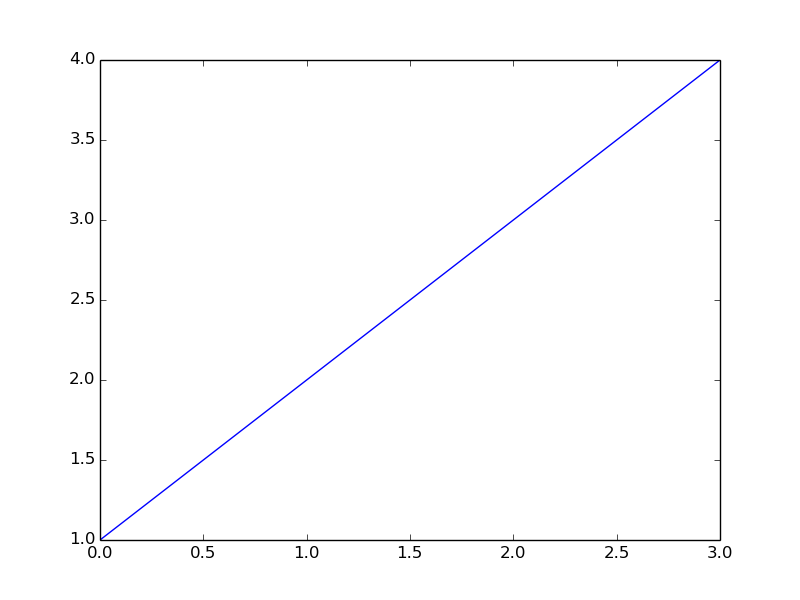
\includegraphics[width=.9\linewidth]{./fig_manual.png}
\end{center}

\item Insert images automatically
\label{sec:orgf269e8f}
\begin{center}
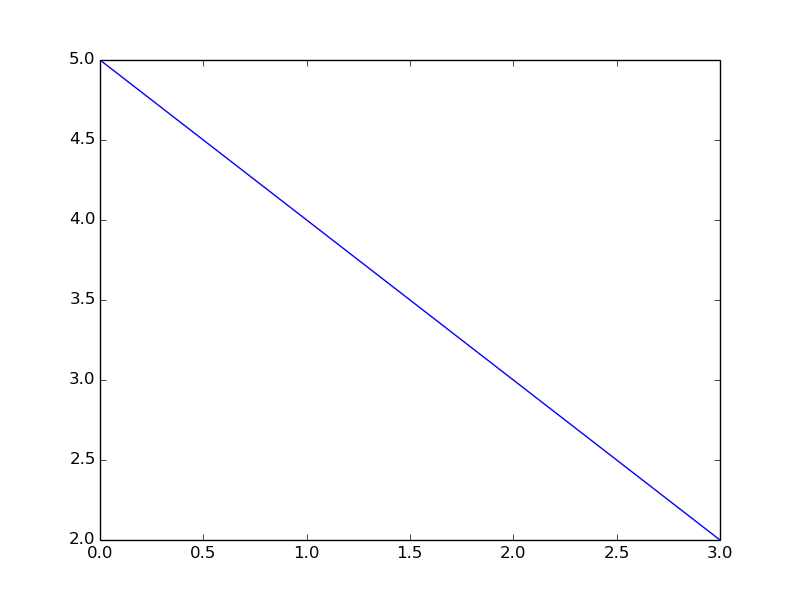
\includegraphics[width=.9\linewidth]{fig_auto.png}
\end{center}
\end{enumerate}


\item R (ggplot2)
\label{sec:orgd4a6ccf}

\begin{center}
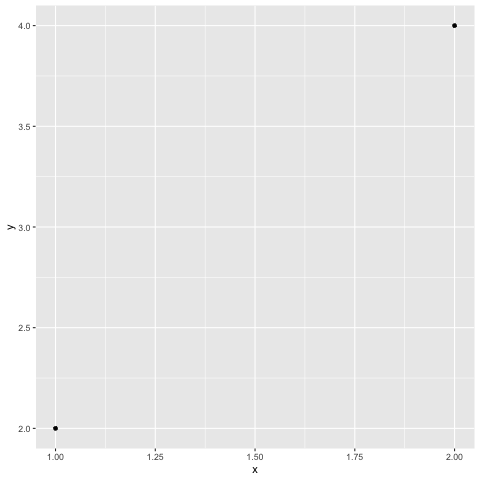
\includegraphics[width=.9\linewidth]{foo.png}
\end{center}

\item C++
\label{sec:org4b0035e}

\begin{enumerate}
\item Hello world!
\label{sec:orga61c626}
\begin{verbatim}
#include <iostream>

int main() {
    std::cout << "Hello World!";
    return 0;
}
\end{verbatim}

\begin{verbatim}
Hello World!
\end{verbatim}


\item Build pyramids
\label{sec:orgd2418cc}
\begin{verbatim}
#include <iostream>
using namespace std;

int main()
{
    int rows = 5;

    for(int i = 1; i <= rows; ++i)
    {
        for(int j = 1; j <= i; ++j)
        {
          cout << j << " ";
        }
        cout << "\n";
    }
    return 0;
}
\end{verbatim}

\begin{center}
\begin{tabular}{rrrll}
1 &  &  &  & \\
1 & 2 &  &  & \\
1 & 2 & 3 &  & \\
1 & 2 & 3 & 4 & \\
1 & 2 & 3 & 4 & 5\\
\end{tabular}
\end{center}
\end{enumerate}
\end{enumerate}
\end{document}